% !TEX root = catron-dissertation.tex
\epstopdfsetup{outdir=./images/02_background/}

\chapter{Literature Review}
\label{chap:02_lit_review}
The literature review will consist of primarily two sections.
The first section will examine aero-optics while the second will look at acoustics inside of ducts.
\section{Aero-Optics}
Optical communication and directed energy systems require a tightly focused beam on target in order to meet system performance objectives.
The farfield performance of airborne optical systems can be degraded by the nearfield flow that becomes optically active at compressible flow speeds.
``Aero-optics'' is the study of the optical effect of these nearfield flow disturbances.
Examples of important aero-optical flows that have been studied extensively include boundary layers \cite{Gordeyev-2014-jcJndkHM,Smith-2013-VXArwwux,Wang-2012-gJ7rttg7}, shear layers \cite{Fitzgerald-2004-DgAgbreK,Rennie-2008-Wku6NheG}, shock waves \cite{Jumper-2013-8KtN3pue}, and even tip vortices \cite{Porter-2013-pQcNWHJ6}.
The effect of acoustic disturbances on aero-optical measurements has also been shown in both flight testing \cite{DeLucca-2018-gBQdjTmT} and ground testing \cite{Catron-2018-DdVp6VZf,Catron-2020-x8njYmmu}.

In these optically active flows the index-of-refraction, $n$, varies locally as does the other fluid properties.
Gladstone and Dale \cite{Gladstone-1863-ND4wtDT9} found that the index-of-refraction is primarily a function of density with a loose dependence on the wavelength of light.
Gladstone and Dale proposed a ``specific refractive energy'' now known as the Gladstone-Dale constant, $K_{GD}$,
\begin{equation}
  K_{GD} = \frac{n-1}{\rho}\textrm{.}
  \label{eqn:02_gladstone_dale_constant}
\end{equation}
For air the refractive index can be related to state quantities \cite{Valley-1965-F3k3cmv6}
\begin{equation}
  n-1 = 77.6\times 10^{-6}\frac{P}{T}\left(1+\frac{7.53\times10^{-3}}{\lambda^2}\right)\textrm{,}
  \label{eqn:02_refractive_index_ptlambda}
\end{equation}
where $P$ is in mbar, $T$ is in K, and $\lambda$ is in $\mu$m.
By combining this relationship with the ideal gas law, the Gladstone-Dale constant can be determined as a function of light wavelength,
\begin{equation}
  K_{GD} = 2.23\times10^{-4}\left(1+\frac{7.53\times10^{-3}}{\lambda_{\mu m}^2}\right) \: \left[\frac{m^3}{kg}\right]\textrm{.}
  \label{eqn:02_gladstone_dale_wavelength}
\end{equation}
The Gladstone-Dale constant for air over the visible range is shown in Figure \ref{fig:02_gladstone_dale_wavelength}.
\begin{figure}
  \centering
  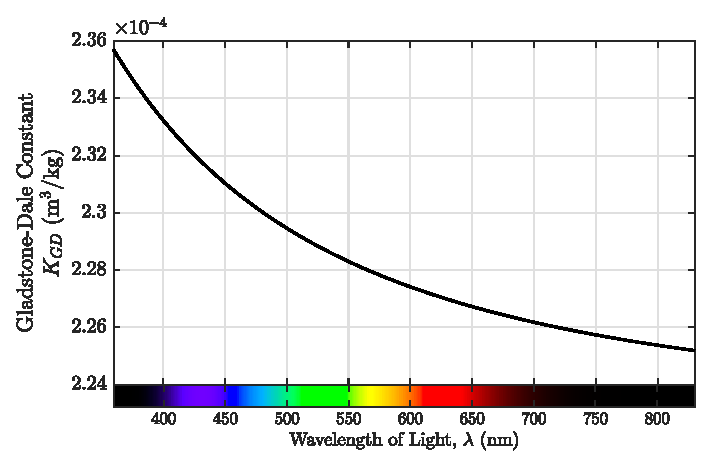
\includegraphics{../matlab/02_background/gladstone_dale_wavelength.eps}
  \caption{Gladstone-Dale constant for air over the visible wavelength range.}
  \label{fig:02_gladstone_dale_wavelength}
\end{figure}
While the value for $K_{GD}$ does vary over the visible range, it is only a few percent, and many sources use an average value of 2.27$\times10^{-4}$ m$^3$/kg for the visible and near-infrared \cite{Gardiner-1980-reW8xrCb}.
The Gladstone-Dale relationship is typically presented as
\begin{equation}
  n = 1+K_{GD}\rho
  \label{eqn:02_gladstone_dale_relation}
\end{equation}
but when applied to situations where there are significant fluctuations in the flow an alternate form is often more useful
\begin{equation}
  n'=K_{GD}\rho'
  \label{eqn:02_gladstone_dale_relation_fluctuating}
\end{equation}
where $'$ denotes the quantity represents the fluctuating component ($n' = n-\bar{n}$).

When a beam with an initially planar wave front passes through a region of optical active flow its wave front aberrated
The optical path length ($\opl$) at any point in the beam can be obtained by integrating the index of refraction along the propagation of an optical ray \cite{Klein-1986-8Vx29RfE}.
\begin{equation}
  \opl (x,y,t) = \int^{s_2}_{s_1} n(x,y,z,t)ds
  \label{eqn:02_opl}
\end{equation}
The optical path difference ($\opd$), is then the spatially-averaged $\textrm{OPL}$ over an aperture removed from the OPL.
\begin{equation}
  \opd(x,y,t) = \opl(x,y,t)-\langle\opl(x,y,t)\rangle
  \label{eqn:02_opd}
\end{equation}
When working with fluctuating components, the $\opd$ can be calculated directly
\begin{equation}
  \opd(x,y,t) = \int^{s_2}_{s_1} n'(x,y,z,t)ds \textrm{.}
  \label{eqn:02_opd_n}
\end{equation}

When $\opd$ is combined with the beam intensity profile, one can compute the farfield complex amplitude distribution using the Fraunhofer approximation \cite{Goodman-1968-zPUmuuzx}.
\begin{equation}
  U(x_0,y_0,t)\propto\iint_{Ap}\exp\left\{\frac{2\pi j}{\lambda}\left[\opd(x_1,y_1,t)-\frac{(x_0x_1+y_0y_1)}{z}\right]\right\}dx_1dy_1
  \label{eqn:02_fraunhofer}
\end{equation}
where $U$ is the complex amplitude, the subscripts 0 and 1 represent the coordinates of the farfield and nearfield respectively.
The intensity can be computed from the complex amplitude via: $I = UU^\ast$.
For cases in which optical aberrations are nonexistent (i.e. $\opd(x,y,t)=0$), the farfield irradiance pattern that results from Equation \ref{eqn:02_fraunhofer} is caused entirely by diffraction from the optical aperture, and is referred to as the “diffraction-limited” irradiance pattern.
For a beam with a flat wave front and circular aperture, the farfield irradiance pattern is the Airy’s disk, and the peak irradiance at the center of the disk, $I_0$ , is the maximum irradiance that can be achieved by the optical system:
\begin{equation}
  I_0 = \left(\frac{kAp^2}{8z}\right)^2
  \label{eqn:02_airy_pattern}
\end{equation}
where $k$ is the wavenumber ($k=2\pi /\lambda$), $Ap$ is the aperture diameter, and $z$ is the distance from the aperture.
In the presence of aero-optical aberrations, $\opd(x,y,t)$ is non-zero, and the farfield irradiance pattern in this case tends to be more spread out and diffuse than the diffraction-limited case; furthermore, the beam may be shifted off target by optical tip/tilt imposed by the aberrations.

The Strehl ratio ($\sr$), is the ratio of intensity on target ($I$) to the diffraction-limited on target intensity ($I_0$):
\begin{equation}
  \sr=\frac{I}{I_0}
  \label{eqn:02_strehl_simple}
\end{equation}
The Strehl ratio can be computed accurately by applying Equation \ref{eqn:02_fraunhofer} twice, once for the diffraction-limited case to obtain $I_0$, and a second time with the $\opd$ field due to aero-optical aberrations included to obtain $I$.
The farfield performance, can also be estimated via the Mar\'{e}chal approximation:
\begin{equation}
  \sr(t) \equiv \frac{I(t)}{I_0} \approx \exp \left\{-\left[\frac{2\pi \opdrms(t)}{\lambda}\right]^2\right\}
  \label{eqn:02_strehl_ratio}
\end{equation}
where $\opdrms$ is the spatial rms of the wave front and $\lambda$ is the wavelength of the beam.
\begin{figure}
  \centering
  \begin{subfigure}[t]{0.45\textwidth}
    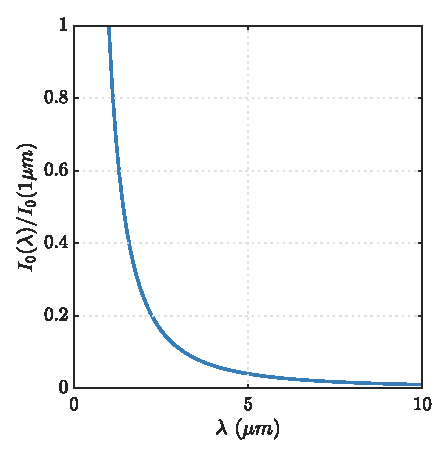
\includegraphics{../matlab/02_background/farfield_intensity.eps}
    \caption{}\label{fig:02_farfield_intensity}
  \end{subfigure}
  ~
  \begin{subfigure}[t]{0.45\textwidth}
    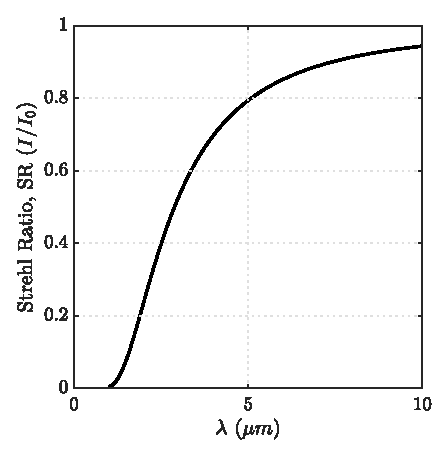
\includegraphics{../matlab/02_background/all_strehl_ratio.eps}
    \caption{}\label{fig:02_all_strehl_ratio}
  \end{subfigure}
  \caption{(\subref{fig:02_farfield_intensity}) Diffraction limited on target intensity as a function of wavelength normalized by the value at $\lambda$ = 1 $\mu$ m. (\subref{fig:02_all_strehl_ratio}) Strehl ratio as a function of wavelength for an aberration that gives SR = 0.95 at $\lambda$ = 10.6 $\mu$m.}
  % \label{FIG:airy_strehl}
\end{figure}
Equation \ref{eqn:02_strehl_ratio} shows a key relationship between $\opd$, wavelength, and the farfield performance, plotted in Figure \ref{fig:02_all_strehl_ratio}.
On the other hand, Equation \ref{eqn:02_airy_pattern} shows that the diffraction-limited farfield irradiance increases as the wavelength is shortened, plotted in Figure \ref{fig:02_farfield_intensity}.
Together, Figure \ref{fig:02_farfield_intensity} and \ref{fig:02_all_strehl_ratio} show that as modern optical systems move to shorter wavelengths to increase $I_0$, aero-optical aberrations cause a much more serious degradation of the Strehl ratio, illustrating why aero-optical considerations are critical in the development of any airborne optical system.

Figure \ref{fig:02_necessary_opd} shows the $\opdrms$ necessary to achieve various Strehl ratios over a range of wavelengths.
\begin{figure}
  \centering
  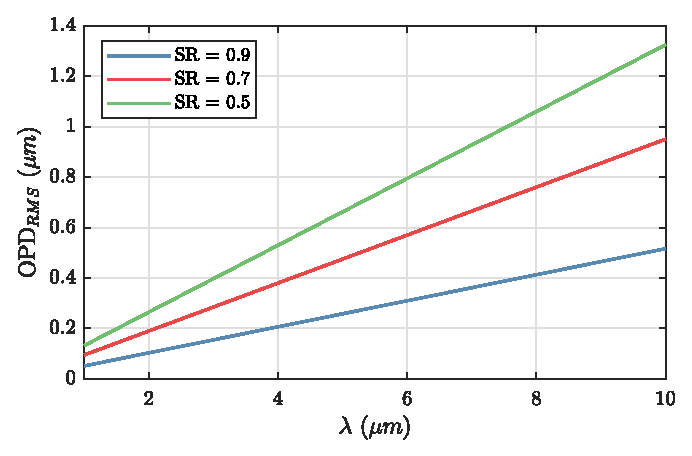
\includegraphics{../matlab/02_background/necessary_opd.eps}
  \caption{$\opdrms$ values necessary to obtain Strehl ratios of 0.9, 0.7, and 0.5 over a range of wavelengths.}
  \label{fig:02_necessary_opd}
\end{figure}
As the wavelength of light decreases the required $\opdrms$ decreases linearly for a fixed Strehl ratio.


\subsection{Typical Optical Wavefront Measurement System}





\begin{figure}
  \centering
  \includegraphics[width=2.5in,clip,trim=200 75 200 75]{../cad/wavefront_setup.pdf}
  \put(-72,62){\rotatebox{90}{\Large LASER}}
  \put(-145,78){\rotatebox{90}{BEAM}}
  \put(-135,65){\rotatebox{90}{EXPANDER}}
  \put(-150,200){\rotatebox{90}{\Large PRIMARY TELESCOPE}}
  \put(-130,400){\rotatebox{90}{\Large MEASUREMENT}}
  \put(-112,427){\rotatebox{90}{\Large REGION}}
  \put(-95,160){\rotatebox{60}{\Large REIMAGING}}
  \put(-80,155){\rotatebox{60}{\Large TELESCOPE}}
  \put(-10,245){\rotatebox{90}{\Large WAVEFRONT}}
  \put(5,260){\rotatebox{90}{\Large SENSOR}}
  \caption{Typical double-pass optical wavefront measurement setup.}
  \label{fig:02_typical_wavefront_system}
\end{figure}




\subsection{A Brief History of Aero-Optics}
The field of aero-optics began with an investigation by Liepmann \cite{Liepmann-1952-89GQ7wyA} into the limits of sensitivity of schlieren systems when used in high-speed flow analysis.
Liepmann used geometric optics to analyze a small-diameter beam and derive its mean-squared fluctuating deflection angle, $\left<\theta^2\right>$.
Liepmann propagated the beam in the $y$ direction and assumed the index of refraction changes in the $x-z$ plane were statistically similar.
Liepmann's analysis for a boundary layer of thickness $\delta$ resulted in
\begin{equation}
  \left<\theta^2\right> = \frac{1}{[n_0(\delta)]^2}\int_0^\delta\int_0^\delta n_0(y)n_0(\zeta)\left<\left(\frac{\partial\nu}{\partial y}\right)^2\right>R_v(|y-\zeta|)dyd\zeta
  \label{eqn:02_liepmann_deflection_angle}
\end{equation}
where the index of refraction is determined from $n=n_0(y)(1+\nu)$ and $R_v(|y-\zeta|)$ is the correlation function for the index variation.
This analysis introduced the concept of a linking equation that allows one to predict time-averaged optical degradation to turbulent flow statistical measurements.

\section{Acoustics}

\subsection{Basic Acoustics}


Starting with the conservation of mass,
\begin{equation}
  \frac{\partial\rho}{\partial t}+\nabla\cdot\left(\rho\mathbf{u}\right)=0  \textrm{,}
  \label{eqn:02_cons_of_mass}
\end{equation}
and separating the density into a time-averaged ($\rho_0$) and fluctuating portion ($\rho'$), $\rho = \rho_0+\rho'$.
The fluctuating conservation of mass equation is obtained by separating the density ($\rho = \rho_0+\rho'$) into a temporally averaged density, $\rho_0$, and a

\begin{equation}
  \frac{\mathbf{D}\rho'}{\mathbf{Dt}}+\nabla\cdot\left(\rho_0\mathbf{u}\right)=0
  \label{eqn:02_cons_of_mass_fluc}
\end{equation}





For acoustics waves of frequency less than $10^9$ Hz the compression of the fluid can be assumed to be adiabatic \cite{Morse-1968-yygEdQZf}.


\begin{equation}
  \left.\frac{\partial p}{\partial\rho}\right|_s = c_0^2
  \label{eqn:02_speed_of_sound}
\end{equation}

\subsection{Duct Acoustics}
Acoustic waves are often enclosed inside of somesort of structure.
This section will look at acoustics when confined to a duct in which the acoustic waves primarily travel along one-axis and have walls confining the acoustics along the other two axes as is the case inside of a wind tunnel.
Figure \ref{fig:02_duct_drawing} shows the diagram used for deriving the acoustic properties inside of a constant area duct.
\begin{figure}
\centering
  % \fbox{
    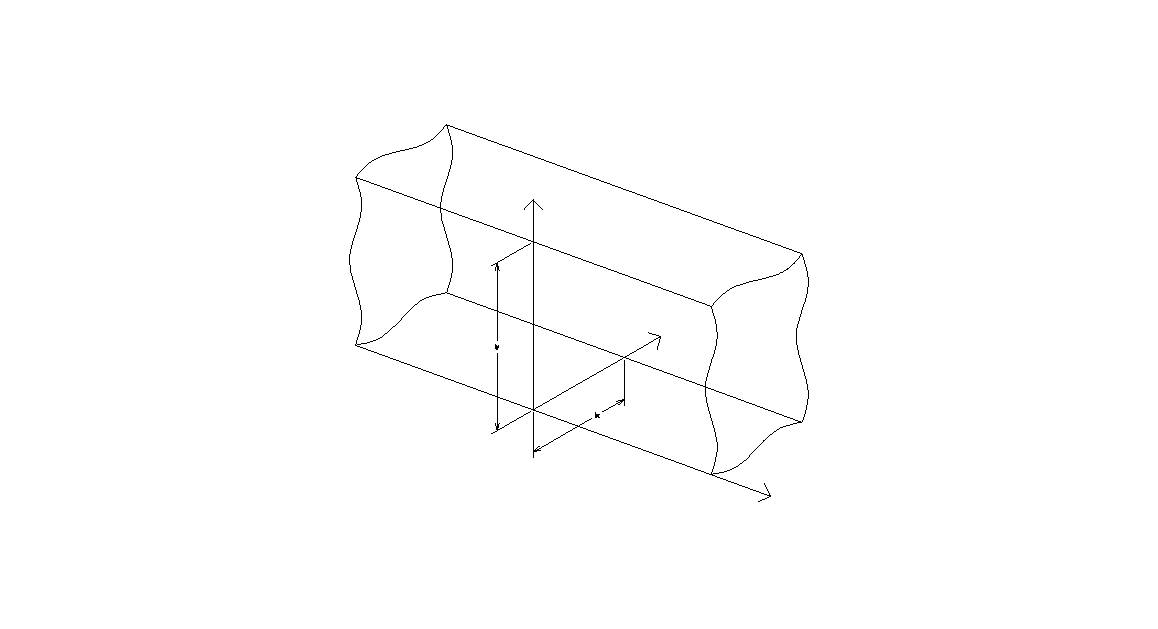
\includegraphics[trim=2.2in 0.7in 2.2in 0.7in,clip,width=4.5in]{../autocad/02_background/duct_drawing.eps}
    \put(-155,62){\fcolorbox{white}{white}{$l_x$}}
    \put(-227,113){\fcolorbox{white}{white}{$l_y$}}
    \put(-103,119){$\mathbf{x}$}
    \put(-198,220){$\mathbf{y}$}
    \put(-26,4){$\mathbf{z}$}
  % }
  \caption{Duct with a rectangular cross-section.}
  \label{fig:02_duct_drawing}
\end{figure}

This derivation is primarily influenced from Munjal \cite{Munjal-2014-w28y4EyP} along with Jacobsen and Juhl \cite{Jacobsen-2013-PHD3v3YZ}.
The primary assumption used in this derivation is that the duct is of constant cross-section.
This means that all mean quantities ($\rho_0$, $\mathbf{u_0}$, ...) a constant throughout space and time.
Starting with the linearized inviscid forms of the conservation of mass,
\begin{equation}
  \frac{\mathbf{D}\rho}{\mathbf{Dt}} + \rho_0\nabla\cdot\mathbf{u} = 0 \textrm{,}
  % \frac{\partial\rho}{\partial t} + \mathbf{u}\cdot\nabla\rho + \rho_0(\nabla\cdot\mathbf{u}) = 0 \textrm{,}
  \label{eqn:02_cons_mass}
\end{equation}
and conservation of momentum,
\begin{equation}
  \rho_0\frac{\mathbf{Du}}{\mathbf{Dt}} + \nabla p = 0 \textrm{.}
  % \rho_0\frac{\partial\mathbf{u}}{\partial t} + \rho_0(\mathbf{u_0}\cdot\nabla)\mathbf{u} + \nabla p = 0 \textrm{.}
  \label{eqn:02_cons_mom}
\end{equation}
The definition of the speed of sound (Equation \ref{eqn:02_speed_of_sound}) is then substituted into Equation \ref{eqn:02_cons_mass},
\begin{equation}
  \frac{1}{c_0^2}\frac{\mathbf{D}p}{\mathbf{Dt}} + \rho_0\nabla\cdot\mathbf{u} = 0 \textrm{,}
  % \frac{1}{c_0^2}\frac{\partial p}{\partial t} + \frac{1}{c_0^2}(\mathbf{u}\cdot\nabla p) + \rho_0(\nabla\cdot\mathbf{u}) = 0 \textrm{,}
  \label{eqn:02_cons_mass_p}
\end{equation}
where $c_0$ is the speed of sound at average fluid properties ($\rho_0$, $p_0$, $T_0$, ...).
Next the difference between the material derivative ($\mathbf{D}/\mathbf{Dt}$) of Equation \ref{eqn:02_cons_mass_p} and the partial derivative ($\partial/\partial\mathbf{x}$) of Equation \ref{eqn:02_cons_mom} with respect to space is taken which results in the convected 3-D wave equation,
\begin{equation}
  \left(\frac{\mathbf{D}^2}{\mathbf{Dt}^2}-c_0^2\nabla^2\right)p=0\textrm{.}
  \label{eqn:02_wave_conv_3_c}
\end{equation}
Expanding the material derivative and dividing by $c_0^2$,
\begin{equation}
  \left(\frac{1}{c_0^2}\frac{\partial^2}{\partial t^2} + \frac{2\mathbf{M}}{c_0}\frac{\partial^2}{\partial t\partial\mathbf{x}} - (1-\mathbf{M}^2)\nabla^2\right)p = 0 \textrm{,}
  \label{eqn:02_wave_conv_expand}
\end{equation}
where $\mathbf{M} = \mathbf{u_0}/c_0$.
By using the fact that $c_0=\omega/k_0$, Equation \ref{eqn:02_wave_conv_3_c} can be written in a more convent form,
\begin{equation}
  \left(\frac{1}{\omega^2}\frac{\partial^2}{\partial t^2} + \frac{2\mathbf{M}}{\omega k_0}\frac{\partial^2}{\partial t\partial\mathbf{x}} - \frac{1-\mathbf{M}^2}{k_0^2}\nabla^2\right)p = 0 \textrm{,}
  \label{eqn:02_wave_conv_3}
\end{equation}
where $\omega$ is the angular frequency and $k_0$ is the total wavenumber.

At this point the pressure field is going to written in a complex form and assumed to be separable in both time and space such that $\hat{p}(\mathbf{x},t) = \hat{p}(x,y)\hat{p}(z)\hat{p}(t)$.
The temporal solution is assumed to take the form
\begin{equation}
  \hat{p}(t) = \exp\left\{j\omega t\right\} \textrm{.}
  \label{eqn:02_pressure_solution_time}
\end{equation}
This results in the spatial component of the convecting wave equation
\begin{equation}
  \left((1-\mathbf{M}^2)\nabla^2-2jk_0\mathbf{M}\nabla+k_0^2\right)\hat{p}(x,y)\hat{p}(z) = 0 \textrm{.}
  \label{eqn:02_wave_conv_space}
\end{equation}
This can be further split into axial and cross-sectional components by splitting $k_0$ into components,
\begin{equation}
  k_0 = \sqrt{k_{xy}^2+k_z^2} \textrm{,}
  \label{eqn:02_k0}
\end{equation}
and because the mean flow is only in the axial direction ($\mathbf{M} = M\mathbf{\hat{k}}$).
The cross-sectional component is a typical Helmholtz equation
\begin{equation}
  \left(\frac{\partial^2}{\partial x^2}+\frac{\partial^2}{\partial y^2}\right)\hat{p}_{xy}(x,y)+k_{xy}^2\hat{p}(x,y) = 0 \textrm{,}
  \label{eqn:02_wave_xy}
\end{equation}
whos solution,
\begin{equation}
  \hat{p}(x,y) = \Psi_m(x,y) \textrm{,}
  \label{eqn:02_pressure_solution_xy}
\end{equation}
is one of infinity many eigen-function solutions with discrete wavenumbers, $k_m$.
The axial component of the convecting wave equation,
\begin{equation}
  (1-M^2)\frac{\partial^2\hat{p}(z)}{\partial z^2} - 2jk_0M\frac{\partial\hat{p}(z)}{\partial z} + k_z^2\hat{p}(z) = 0 \textrm{,}
  \label{eqn:02_wave_z}
\end{equation}
retains the total wavenumber in second term which means its solution will depend on the cross-sectional wavenumber value at cross-sectional mode.
The solution to the axial convecting wave equation,
\begin{equation}
  \hat{p}(z) = p^+_m\exp{\left\{-jk^+_{zm}z\right\}}+p^-_m\exp{\left\{+jk^-_{zm}z\right\}} \textrm{,}
  \label{eqn:02_pressure_solution_z}
\end{equation}
has waves traveling in both directions with the axial wavenumber in each direction for a given mode
\begin{equation}
  k^\pm_{zm} = \frac{\mp Mk_0+\sqrt{k_0^2-(1-M^2)k_m^2}}{1-M^2} \textrm{.}
  \label{eqn:02_kzm}
\end{equation}

The solution for a three-dimensional acoustic wave in a duct with a constant but arbitrary cross-section in complex pressure is the combination of the component solutions presented in Equations \ref{eqn:02_pressure_solution_time}, \ref{eqn:02_pressure_solution_xy}, and \ref{eqn:02_pressure_solution_z},
\begin{equation}
  \hat{p}(x,y,z,t) = \Psi_m(x,y)\left(p^+_m\exp{\left\{-jk^+_{zm}z\right\}}+p^-_m\exp{\left\{+jk^-_{zm}z\right\}}\right)\exp\left\{j\omega t\right\} \textrm{.}
  \label{eqn:02_pressure_solution_duct}
\end{equation}
The two solutions for a plane wave ($\Psi_m=1$, $k_m=0$) traveling in a duct have a characteristic speed of $u\pm c_0$.
Acoustic modes will travel indefinitly if $k_0^2-(1-M^2)k_m^2>0$ (the quantity inside of the square-root of Equation \ref{eqn:02_kzm}).
This presents a frequency at which a given mode will cut-on,
\begin{equation}
  f_{cuton} = \frac{c_0}{2\pi}\sqrt{(1-M^2)k_m^2} \textrm{.}
  \label{eqn:02_cuton_freq}
\end{equation}
Below this frequency, an acoustic mode will be exponentially attenuated as it travels throught the duct.

\subsubsection{Characteristic Equations of Cross-Sections}
In order to determine the characteristic equations of an acoustic field within a cross-section the solution to Equation \ref{eqn:02_wave_xy} needs to be determined.
A typical boundary condition that is used in the solution of this 2-D Helmholtz equation is using the assumption that the walls are rigid.
\begin{equation}
  \nabla p_{x,y}(x,y)\cdot\mathbf{n}_{wall} = 0
  \label{eqn:02_bc_rigig_wall}
\end{equation}
This boundary condition results in the acoustic waves being perfectly reflected off of the duct walls.
There are several known empirical solution sets of the characteristic equations for specific geometry with the rigid wall assumption.

The first of these solutions is for a rectangular cross-section,
\begin{equation}
  \Psi_{m,n}(x,y) = \cos(k_xx)\cos(k_yy) \textrm{,}
  \label{eqn:02_psi_rect}
\end{equation}
where the wave numbers along each axis are $k_x = m\pi/l_x$ and $k_y = n\pi/l_y$.
The duct has a width of $l_x$ and a height of $l_y$.
The total cross-sectional wave number for use in determining the axial wave numbers is
\begin{equation}
  k_m^2 = k_x^2+k_y^2 \textrm{.}
  \label{eqn:02_wave_number_crosssection}
\end{equation}
Figure \ref{fig:02_cross_section_rect} shows the characteristic functions when m=0:2 and n=0:3 for a rectangular cross-section of width of $l_x$ and height of $l_y$.
\begin{figure}
  \centering
  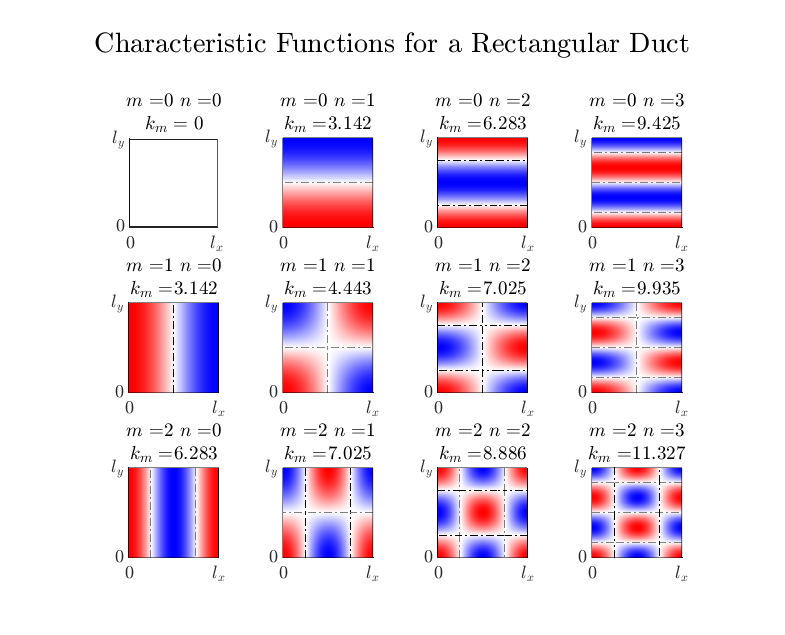
\includegraphics{../matlab/02_background/cross_section_rect.eps}
  \caption{Characteristic solutions to Equation \ref{eqn:02_wave_xy} with rigid wall in a rectangular cross-section where m=0:2 and n=0:3.  Nodal lines are depicted by the dot-dash lines.  The cross-sectional wave numbers, $k_m$, listed are for a duct of unit length and height.}
  \label{fig:02_cross_section_rect}
\end{figure}
The lines depicted in the figure are nodal lines and represent locations where there is zero pressure fluctuations for that acoustic mode.

The second set of known empirical solutions is for a circular cross-section with radius $R$,
\begin{equation}
  \Psi_{m,n}(r,\theta) = J_m(k_{mn}r)\exp\left\{\pm jm\theta\right\} \textrm{,}
  \label{eqn:02_psi_circ}
\end{equation}
where $J_m$ is the $m^\textrm{th}$ Bessel function of the first kind and the $\pm$ indicates the direction of spin.
If the left and right spin coefficients are equal in magnitude then a non-spinning mode is created.
In order to satisfy the solid wall boundary condition $J_m'(k_{mn}R) = 0$ which determines a set of discrete values for the cross-sectional wave number at the $n^\textrm{th}$ zero for the $m^\textrm{th}$ Bessel function.
Figure \ref{fig:02_cross_section_circ} shows the characteristic functions for a circular duct.
\begin{figure}
  \centering
  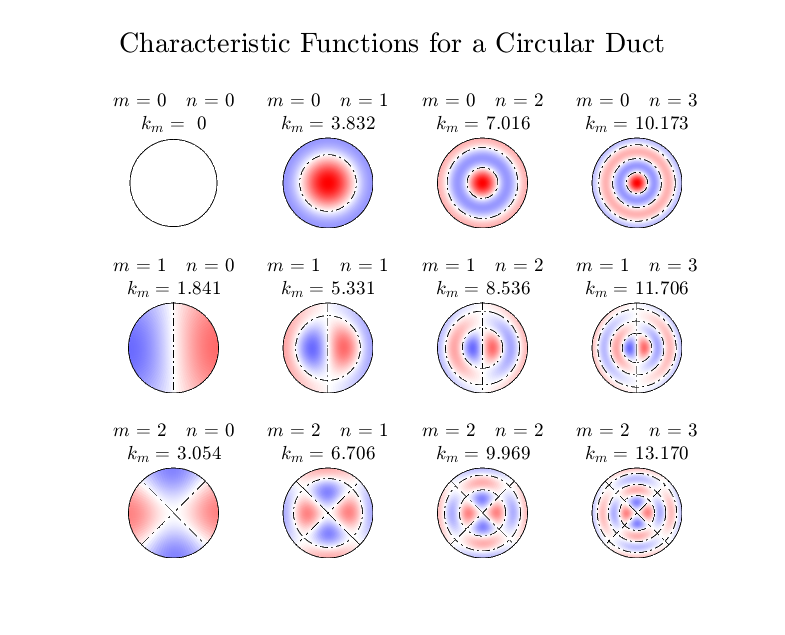
\includegraphics{../matlab/02_background/cross_section_circ.eps}
  \caption{Characteristic solutions to Equation \ref{eqn:02_wave_xy} with rigid wall in a circular cross-section where m=0:2 and n=0:3.  Nodal lines are depicted by the dot-dash lines.  The cross-sectional wave numbers, $k_m$, listed are for a duct of unit radius.}
  \label{fig:02_cross_section_circ}
\end{figure}
